\subsection{PRBS tests}

\paragraph{Test 1.} Follow the following steps:
\begin{enumerate}
    \item Configure the GBTx slave to send PRBS data. Write ``03151515'' to
        slave register \texttt{0x1c}, setting size to 4.
    \item Go to the top MiniDAQ hardware panel, click on \textbf{PRBS}.
    \item In the \textbf{PRBS} panel, click in sequence:
        \textbf{Stop All Generators} $\to$ \textbf{Reset All Counters} $\to$
        \textbf{Start All Generators} $\to$ \textbf{Start All Checkers} $\to$
        \textbf{Start All Counters}.
\end{enumerate}

The result should be the same as shown in \autoref{fig:prbs-test1}.

\begin{figure}[ht]
    \centering
    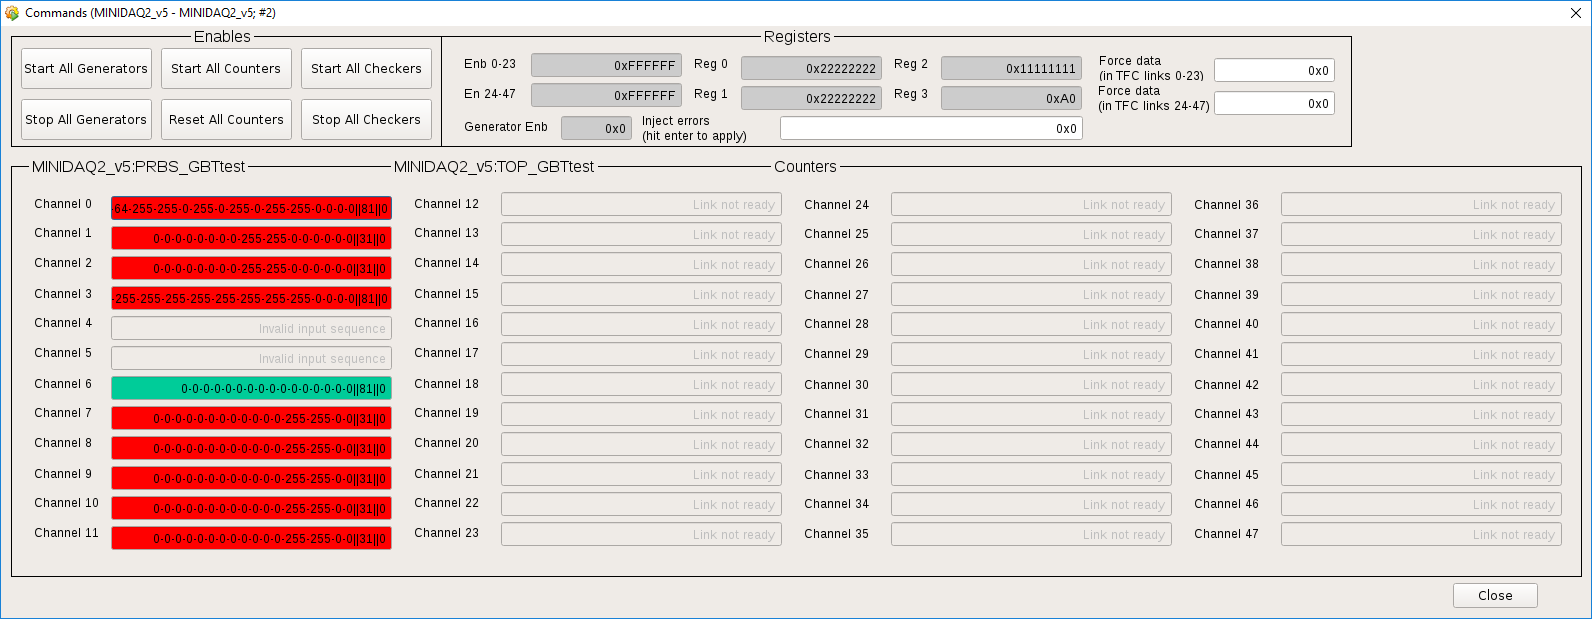
\includegraphics[width=\textwidth]{res/prbs_test1.png}
    \caption{Expected result for PRBS test 1.}
    \label{fig:prbs-test1}
\end{figure}

\begin{leftbar}
    Channel 6 (optical fiber 11, which is connected to slave GBTx) should go
    green and show a bunch of 0s.
    These 0s are the PRBS nibbles (7 bits) each from the GBT.
\end{leftbar}

\begin{leftbar}
    Channel 7 or any other channels should go red and show a lot of errors,
    because these are receiving the FE data in loopback and not the ``correct''
    random data that the checkers are expecting.
\end{leftbar}

\paragraph{Test 2.} Follow the following steps:
\begin{enumerate}
    \item Configure the GBTx slave to send PRBS data. Write ``00171717'' to
        slave register \texttt{0x1c}, setting size to 4.
    \item Go to the top MiniDAQ hardware panel, click on \textbf{PRBS}.
    \item In the \textbf{PRBS} panel, click in sequence:
        \textbf{Stop All Generators} $\to$ \textbf{Reset All Counters} $\to$
        \textbf{Start All Generators} $\to$ \textbf{Start All Checkers} $\to$
        \textbf{Start All Counters}. (same as in test 1).
\end{enumerate}

The result should be the same as shown in \autoref{fig:prbs-test2}.

\begin{figure}[ht]
    \centering
    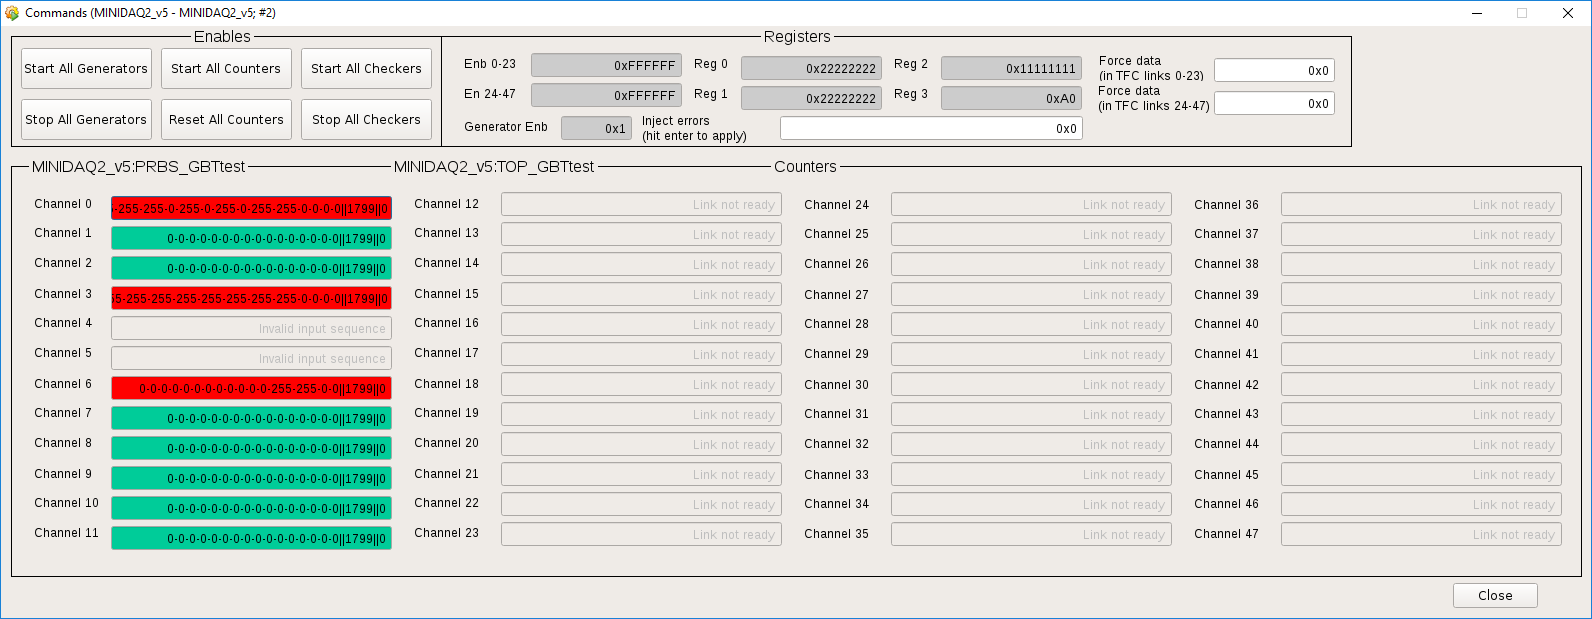
\includegraphics[width=\textwidth]{res/prbs_test2.png}
    \caption{Expected result for PRBS test 2.}
    \label{fig:prbs-test2}
\end{figure}

\begin{leftbar}
    All channels that are in loopback should go green: Now the PRBS data is
    generated inside FPGA, it overwrites the FE data and goes back in loopback
    to the checkers.
\end{leftbar}

\begin{leftbar}
    Channel 6  shows counting errors on two nibbles.
    The reason, according to expert Federico Alessio, is the clock-crossing
    domain inside the GBTx chip that generates errors in the loopback path,
    which is a feature of the GBT.
\end{leftbar}

\begin{leftbar}
    The increasing counter to the right of each line in the PRBS block is the
    number of seconds since we started the counters.
\end{leftbar}

\begin{leftbar}
    To have again FE data we need to disable the generators:
    \textbf{Stop All Generators} in the \textbf{PRBS} panel.
\end{leftbar}

\begin{leftbar}
    When the PRBS panel shows ``Input data not valid'', it means that the
    system is generating all 0s.
\end{leftbar}
